\chapter{From Spike Trains to Node Embeddings: A Reservoir-to-Graph Representation Pipeline}
\label{chap:embeddings}

\section{Introduction: From Reservoir Output to Fixed-Length Features}
\label{sec:ch4_intro}

Given the provisional operating point from Chapter~\ref{chap:lsm}, this chapter compares ways to convert a sparse spike matrix into a fixed-length vector. The comparison asks how mean rate, latency, and binned counts behave on a controlled temporal-pattern task, and how much dimensionality can be removed without a large loss in readout accuracy. A bin index has explicit temporal meaning; a principal component, by contrast, is a data-dependent linear combination and requires more cautious interpretation.

Many spike-train summaries are available, but there is no single representation that is optimal for every task. Here the purpose is narrower: specify one reproducible feature pipeline, compare it with plausible alternatives on synthetic data, and disclose what the comparison does and does not establish for the later graph analysis.

Chapter~\ref{chap:lsm} showed amplitude-dependent spikes in one selected realization and a window-dependent mean-rate contrast for two deterministic pulse responses. This chapter uses a separate, noisy synthetic task with timing and amplitude jitter to make the feature comparison less trivial.

For the synthetic experiments and the audited rerun specification, one channel produces a binary spike matrix $\mathbf{S} \in \{0, 1\}^{N_{\text{res}} \times T}$ with $N_{\text{res}}=256$ units and $T=60$ steps from the early window (steps 10--70). This is a 15,360-element object indexed by unit and time. A graph readout requires a fixed-length vector $\mathbf{h}_v^{(0)} \in \mathbb{R}^d$ for each node. The summary from $\mathbf{S}$ to $\mathbf{h}_v^{(0)}$ determines which temporal distinctions remain available to that readout.


\section{Background: Neural Coding}
\label{sec:neural_coding_theory}

The question of how to extract a feature vector from a spike train is a specific instance of the \emph{neural coding problem}, one of the foundational questions in computational neuroscience. The debate concerns what aspects of a neural spike train carry information about the stimulus: the overall firing rate (rate coding), the precise timing of individual spikes (temporal coding), or some combination \cite{gerstner_spiking_2002, dayan2001, Rieke1997}.

This distinction is relevant to the feature comparison: if mean firing rate supports the selected readout, finer bins may be unnecessary for this task; if binned counts perform better, the ordering of activity within the window is useful to that readout.

The data-processing inequality states that a deterministic summary cannot increase mutual information with the label. No mutual information or statistical sufficiency is estimated here. Cross-validated readout accuracy is instead used as a task-specific measure of accessibility, and retained PCA variance is reported as a separate compression summary.

\subsection{An Evaluation Task: Temporal Pattern Discrimination}

The controlled task presents three sub-pulses with strong--medium--weak amplitudes for Class~0 and the reverse order for Class~1. The nominal profiles contain the same set of amplitudes, but independent amplitude and timing jitter plus additive Gaussian noise mean that realized trial energy is not exactly matched. The executable configuration uses noise standard deviation 0.5, amplitude jitter of $\pm30\%$, timing jitter of $\pm5$ steps, 200 generated observations per class, and random seed 42. Consequently, performance differences are evidence about these feature/readout combinations on this generator, not proof that only temporal order distinguishes every realized observation.


\section{Reservoir Size Ablation}
\label{sec:size_ablation}

Reservoir size changes both feature dimension and computational cost. The BSC$_6$--PCA-64--logistic pipeline was evaluated for $N_{\text{res}}\in\{64,128,256,512\}$ using five fixed stratified splits. Scaling and PCA were fitted only on each training fold and applied to its held-out fold.

The fold accuracies are shown in Figure~\ref{fig:reservoir_size_ablation}. The differences are small for this synthetic generator. No valid hypothesis test was performed on the five correlated fold scores, so the result is used to select 256 units as a cost--accuracy compromise rather than to claim statistical equivalence or a universal saturation point.

\begin{figure}[H]
    \centering
    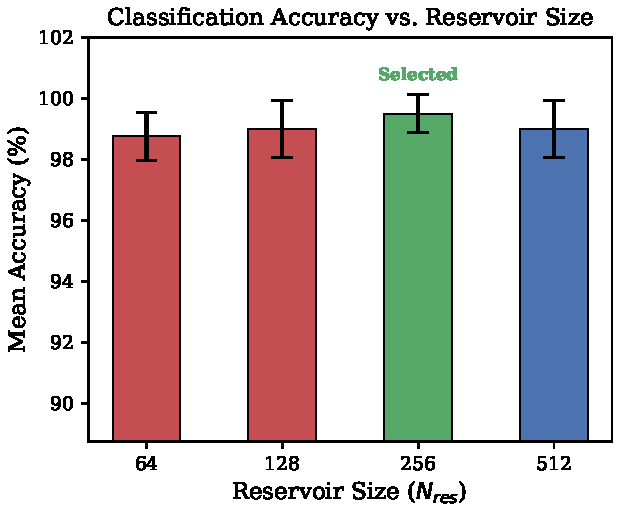
\includegraphics[width=0.65\textwidth]{pictures/chLSMEmbeddings/ablation_reservoir_size.pdf}
    \caption{Mean held-out-fold accuracy versus reservoir size. Scaling and PCA were fitted within each training fold; error bars are the standard deviation across five correlated folds and are not confidence intervals.}
    \label{fig:reservoir_size_ablation}
\end{figure}


\section{Descriptive Comparison of Representation Geometry}
\label{sec:separability}

\subsection{Fisher Discriminant Ratio with Regularization}

The Fisher Discriminant Ratio (FDR $=\operatorname{tr}(\mathbf{S}_W^{-1}\mathbf{S}_B)$) summarizes between-class relative to within-class scatter \cite{duda_pattern_2001}. For the 1536-dimensional BSC$_6$ vectors with 200 samples per class, $\mathbf{S}_W$ is rank-deficient (rank $\leq398<1536$). Tikhonov regularization was applied as $\mathbf{S}_W\leftarrow\mathbf{S}_W+\epsilon\mathbf{I}$ with $\epsilon=10^{-4}\operatorname{tr}(\mathbf{S}_W)/d$. The same rule was used for each representation, but differing dimensions and spectra still limit direct ratio comparisons.

\subsection{Results and Limits of the FDR Comparison}

The regularized FDR comparison in Figure~\ref{fig:fdr_comparison} gives the following descriptive values:
\begin{itemize}
    \item Raw input (binned): FDR = 0.13
    \item Linear filter (5-point moving average + binning): FDR = 0.13
    \item LSM reservoir (BSC$_6$): FDR = 1158
\end{itemize}

The numerical ratio is approximately $8{,}900$, but it should not be interpreted as an effect-size ratio or a causal decomposition. The representations have different dimensions and covariance spectra, and the regularized inverse is sensitive to the chosen $\epsilon$ in this rank-deficient setting. Moreover, a single moving-average baseline does not isolate thresholding, recurrence, and expansion. The comparison shows that this particular regularized statistic is much larger for BSC$_6$ than for the two stated baselines; it does not show which reservoir mechanism caused the difference.

\begin{figure}[H]
    \centering
    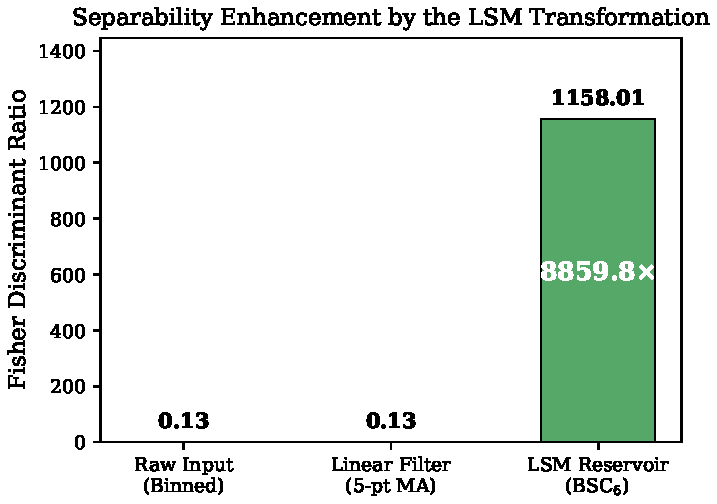
\includegraphics[width=0.7\textwidth]{pictures/chLSMEmbeddings/fdr_three_way_comparison.pdf}
    \caption{Regularized Fisher ratio for raw binned input, a five-point moving-average baseline, and BSC$_6$. Values are descriptive and are sensitive to dimension, covariance rank, and the regularization rule; they do not identify a causal contribution of reservoir components.}
    \label{fig:fdr_comparison}
\end{figure}


\section{Comparative Analysis of Neural Coding Representations}
\label{sec:coding_comparison}

\subsection{Design and Results}

Four coding schemes were compared, each evaluated with both logistic regression and SVM-RBF classifiers (Table~\ref{tab:coding_results}, Figure~\ref{fig:coding_comparison}).

\begin{table}[H]
    \centering
    \caption{Mean held-out-fold accuracy (\%) for each coding scheme on the synthetic temporal-pattern generator. Preprocessing was fitted within each training fold. Error terms are fold standard deviations, not confidence intervals.}
    \label{tab:coding_results}
    \begin{tabular}{|l|c|c|}
        \hline
        \textbf{Coding Scheme} & \textbf{Logistic Regression} & \textbf{SVM (RBF)} \\
        \hline
        Mean Firing Rate (MFR) & $47.5\% \pm 4.1\%$ & $51.2\% \pm 4.9\%$ \\
        Latency to First Spike (LFS) & $70.0\% \pm 4.4\%$ & $70.8\% \pm 3.3\%$ \\
        BSC (3 Bins) & $98.3\% \pm 1.3\%$ & $98.3\% \pm 1.3\%$ \\
        \textbf{BSC (6 Bins)} & $\mathbf{99.5\% \pm 0.6\%}$ & $\mathbf{99.5\% \pm 0.6\%}$ \\
        \hline
    \end{tabular}
\end{table}

\begin{figure}[H]
    \centering
    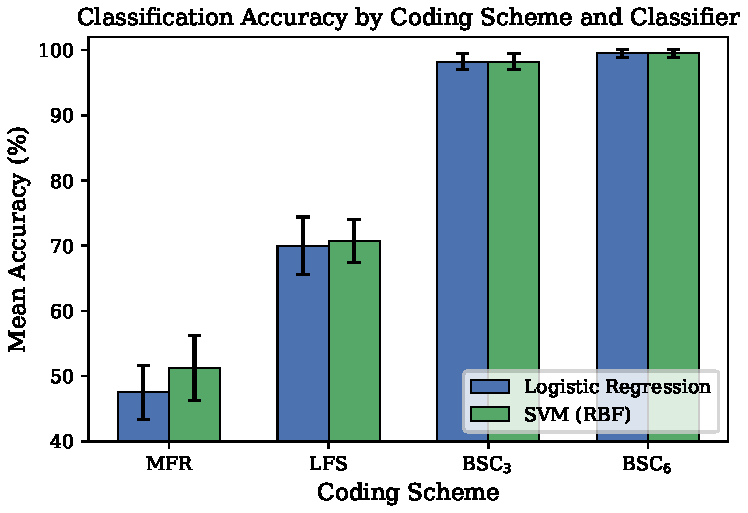
\includegraphics[width=0.65\textwidth]{pictures/chLSMEmbeddings/coding_scheme_accuracy_comparison.pdf}
    \caption{Held-out-fold accuracy by coding scheme and classifier. BSC$_6$ performs substantially better than MFR on this generator, showing that within-window binning is useful to these readouts; it does not establish that all label information is exclusively temporal.}
    \label{fig:coding_comparison}
\end{figure}

An additional comparison with inter-spike interval histograms and the Victor--Purpura distance \cite{victor_purpura_1996} reported 99.7\% accuracy at more than 50 times the measured computation. Because performance is near the ceiling and timing depends on the implementation and hardware, this is a practical comparison for the recorded experiment rather than proof of an optimal code.

\subsection{Interpretation of the Coding Comparison}

The MFR logistic-regression result is close to chance for this balanced generator. It indicates that the selected linear readout could not use mean-rate features reliably under these splits. It does not establish zero mutual information, and the realized noisy stimuli are not exactly energy matched.

The BSC$_6$ result shows that six 10-step counts make the generated early-versus-late pattern highly accessible to both selected readouts. Relative to MFR, the representation retains coarse ordering within the 60-step window. The comparison does not exclude contributions from realized amplitude, timing, or noise differences.

First-spike latency gives intermediate accuracy. This is consistent with sensitivity to early timing while discarding later events, although the experiment does not isolate the exact source of its errors.

The large accuracy gap supports BSC$_6$ for the subsequent pipeline. Its magnitude is specific to this generator and should not be projected onto SHAPE EEG without a direct, fold-safe comparison there.

Each BSC$_6$ feature has an explicit neuron and 10-step-bin index, whereas mean rate collapses the full window. This makes the pre-PCA code temporally traceable. Once PCA mixes neurons and bins, that one-to-one feature interpretation no longer holds.


\section{Dimensionality Reduction, Representational Geometry, and Robustness}
\label{sec:pca_robustness}

\subsection{PCA Compression}

PCA was applied to the 1536-dimensional BSC$_6$ vectors. The full-data eigenspectrum is shown descriptively in Figure~\ref{fig:pca_variance}: 64 components account for 50.5\% of total sample variance. For every accuracy estimate, standardization and PCA were refitted inside each training fold before transforming the held-out fold. With that procedure, PCA-64 retained $99.5\%\pm0.6\%$ accuracy, and PCA-5 also yielded $99.5\%\pm0.6\%$ on this generator. These near-ceiling values show that five training-fold principal components were sufficient for the selected readout; they do not prove a unique intrinsic dimension.

PCA is unsupervised, so explained variance alone does not identify class-discriminating directions. The combination of a long eigenspectrum tail and high fold-safe accuracy after compression supports PCA as a practical size reduction for this synthetic dataset. It does not establish that discarded variance is nuisance, and there is no biological variability in the generator.

\begin{figure}[H]
    \centering
    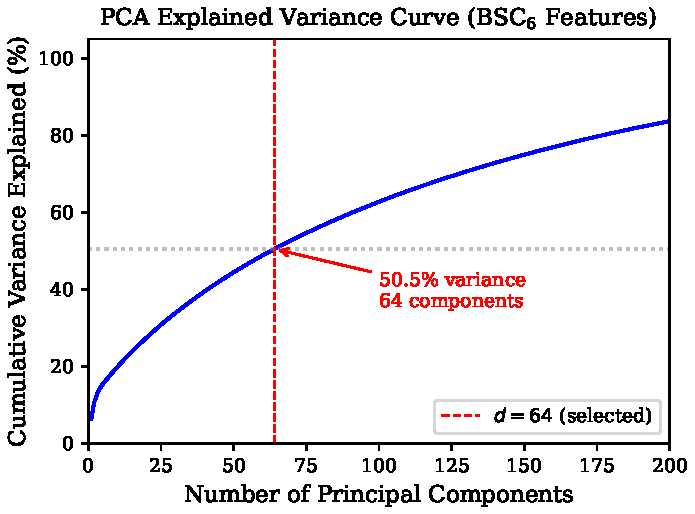
\includegraphics[width=0.65\textwidth]{pictures/chLSMEmbeddings/pca_explained_variance.pdf}
    \caption{Full-sample cumulative explained variance for BSC$_6$. Accuracy at each component count was evaluated separately with fold-fitted PCA; five components were sufficient for near-ceiling readout accuracy on this generator.}
    \label{fig:pca_variance}
\end{figure}

\subsection{Interpretation of Principal Component Structure}

Figure~\ref{fig:pca_components} averages each full-data component's signed loadings across neurons within each of the six bins. The display is an exploratory temporal summary: PCA signs are arbitrary, averaging can hide heterogeneous neuron loadings, and no supervised statistic establishes that a particular component is a primary class discriminator.

The profiles show that the leading components mix contributions from several time bins. They may help inspect the compression globally, but individual PCA coordinates should not be assigned fixed semantic labels such as onset or relative timing without stability and loading-level analyses. The downstream model receives numerical coordinates, not guaranteed disentangled concepts.

\begin{figure}[H]
    \centering
    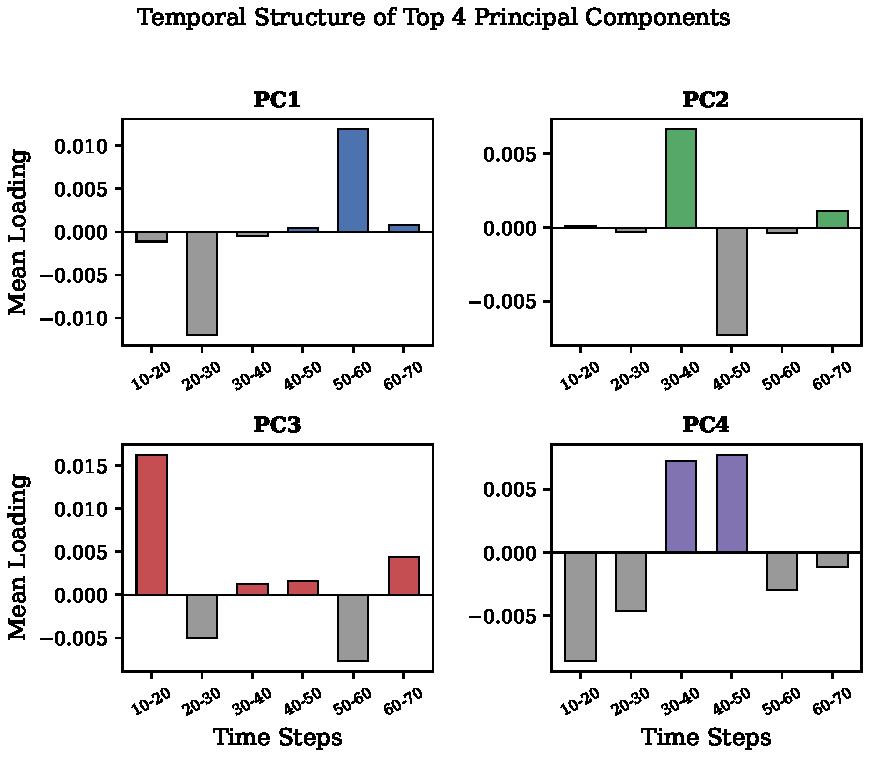
\includegraphics[width=0.9\textwidth]{pictures/chLSMEmbeddings/pca_component_visualization.pdf}
    \caption{Exploratory temporal profiles of the top four full-data principal components, computed by averaging signed loadings across neurons within each bin. Component signs are arbitrary and the averages do not provide functional labels.}
    \label{fig:pca_components}
\end{figure}

\subsection{Cross-Initialization Robustness}

Across 10 reservoir initializations, BSC$_6$+PCA-64 yielded mean fold-averaged accuracy of $99.3\%\pm0.3\%$ across seeds, while MFR yielded $50.8\%\pm2.7\%$ (Figure~\ref{fig:robustness}). PCA and scaling were fitted within each training fold. The reported standard deviations describe variation across these 10 seeds, not uncertainty for an unrestricted population of reservoirs.

The seed sweep shows stable task accuracy for the synthetic generator. It does \emph{not} show that independently initialized reservoirs or independently fitted PCA bases produce coordinate-wise comparable node features. That distinction matters for graph inputs and motivates the common, fold-fitted basis specified in the corrected Chapter~\ref{chap:arspi_net} analysis code.

\begin{figure}[H]
    \centering
    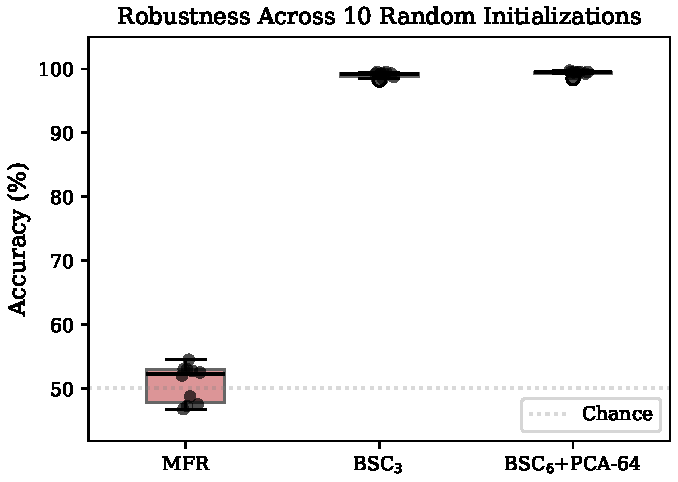
\includegraphics[width=0.55\textwidth]{pictures/chLSMEmbeddings/cross_initialization_robustness.pdf}
    \caption{Fold-averaged accuracy across 10 reservoir initializations. Each dot is one seed; transforms were fitted inside each training fold. Stability of accuracy does not imply alignment of feature coordinates across seeds.}
    \label{fig:robustness}
\end{figure}

\subsection{Parameter Sensitivity}

The pipeline was also evaluated over the finite grid $\beta\in\{0.03,\ldots,0.08\}$ and $M_{\text{th}}\in\{0.3,\ldots,0.7\}$ (Figure~\ref{fig:sensitivity}), with fold-fitted preprocessing. High accuracy throughout this grid shows low sensitivity for the synthetic generator and sampled values; it does not validate transfer to different input statistics.

\begin{figure}[H]
    \centering
    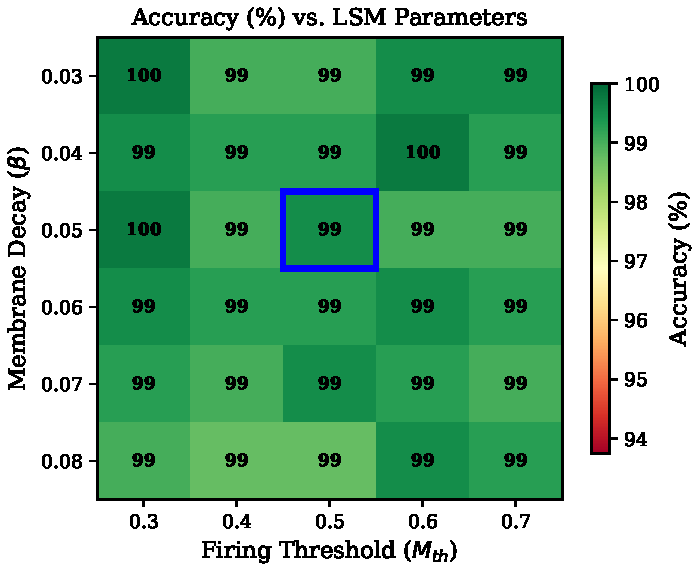
\includegraphics[width=0.6\textwidth]{pictures/chLSMEmbeddings/parameter_sensitivity_heatmap.pdf}
    \caption{BSC$_6$+PCA-64 held-out-fold accuracy across the sampled $\beta$ and threshold grid. Results describe this generator and finite grid only.}
    \label{fig:sensitivity}
\end{figure}


\section{Chapter Synthesis: Provisional Embedding Specification}
\label{sec:ch4_synthesis}

\subsection{Summary of Findings}

The synthetic experiments support the following limited conclusions:

\begin{enumerate}
    \item \textbf{Representation geometry differs}: The regularized FDR is much larger for BSC$_6$ than for the raw and moving-average baselines. Dimension, covariance, and regularization prevent a causal or effect-size interpretation of the $8{,}900\times$ numerical ratio.

    \item \textbf{Coarse temporal binning helps on this task}: BSC$_6$ substantially outperforms MFR for the noisy early-versus-late generator. Each pre-PCA bin maps to a specified response interval, but no mutual-information claim follows.

    \item \textbf{Fold-fitted compression preserves synthetic-task accuracy}: PCA-64 retains near-ceiling accuracy when fitted inside each training fold. PCA coordinates mix bins and neurons and therefore do not preserve a one-feature/one-window interpretation.

    \item \textbf{Accuracy is stable over the tested settings}: BSC$_6$+PCA-64 yields $99.3\%\pm0.3\%$ across 10 seeds and high accuracy over the sampled parameter grid. This does not establish coordinate alignment or real-data robustness.
\end{enumerate}

\subsection{Final Embedding Specification}

\begin{table}[H]
    \centering
    \caption{Audited specification for a corrected real-data rerun. PCA must be fitted on training data only and shared across channels when coordinates are compared.}
    \label{tab:final_embedding_spec}
    \renewcommand{\arraystretch}{1.2}
    \begin{tabular}{|l|p{8cm}|}
        \hline
        \textbf{Parameter} & \textbf{Specification} \\
        \hline
        Reservoir size ($N_{\text{res}}$) & 256 neurons \\
        Membrane decay ($\beta$) & 0.05 \\
        Firing threshold ($M_{\text{th}}$) & 0.5 \\
        Feature window & Time steps 10--70 post-stimulus \\
        Coding scheme & BSC$_6$ (6 bins $\times$ 10 steps each) \\
        Dimensionality reduction & PCA, 64 components \\
        Evaluation rule & Fit scaling and one common PCA basis on each training fold only; transform held-out data without refitting \\
        \textbf{Output} & $\mathbf{h}_v^{(0)} \in \mathbb{R}^{64}$ per channel index \\
        \hline
    \end{tabular}
\end{table}

\subsection{Scope and Transfer Considerations}

The pipeline was selected on synthetic stimuli. The audit found three mismatches in the archived SHAPE workflow. PCA was fitted globally and, in some scripts, separately by channel. The primary Chapter~5 extractor divided the full 256-sample post-stimulus epoch into six 42-sample bins and dropped the final four samples, rather than using steps 10--70; the later temporal-traceability analysis did use the early window. Finally, the primary script initialized different random reservoir weights for each channel. Equal-numbered neuron features therefore did not share a common transformation across graph nodes. Thus the primary Chapter~5 embedding and the early-window attention analysis are different representations despite sharing the BSC$_6$ label, and the archived node coordinates were misaligned before PCA.

The corrected source applies one saved reservoir to every channel, uses steps 10--70, standardizes on the training fold, and fits one common PCA basis inside that fold. Raw SHAPE inputs were not included in the audited source package, so this corrected real-data analysis could not be rerun. Archived numerical results remain descriptive and do not validate the specification in Table~\ref{tab:final_embedding_spec}.

\subsection{Exploratory Temporal Traceability Check}
\label{sec:ch4_temporal_traceability}

Temporal traceability is used here in a narrow operational sense: every uncompressed BSC$_6$ value has a known response interval. The following archived profile correlations are exploratory comparisons with conventional ERP summaries, not validation that an early spike bin measures an ERP component.

Per-channel means were formed for six early intervals (39--78, 78--117, 117--156, 156--195, 195--234, and 234--273~ms) from the archived centered summaries ($N=211$ subjects; 633 subject--condition observations). The archived profile analysis reported $r=0.65$ against a P300 summary (250--500~ms) and $|r|=0.82$ against an LPP summary (500--800~ms), with a largest channel-wise value of $r=0.837$ for Channel~31. These correlations compare aggregate profiles; they are not subject-level recovery statistics. The BSC intervals overlap only the beginning of the stated P300 window and do not overlap the LPP window, so the associations cannot establish direct temporal correspondence with either full component.

The values show covariation among aggregate summaries that may share condition or channel structure. They do not show that early bins recover the P300 or LPP, do not provide a patient-level $R^2$, and do not establish clinical utility \cite{nelson_hajcak_2017}.

An archived temporal-resolution sweep reported:
\begin{center}
\begin{tabular}{lcccc}
\toprule
\textbf{Bins} & \textbf{Resolution} & \textbf{Accuracy} & \textbf{Peak Bin} & \textbf{Peak Acc.} \\
\midrule
6 & 39.1~ms & $67.0\% \pm 5.4\%$ & Bin 6 (234--273~ms) & $68.1\%$ \\
12 & 19.5~ms & $65.9\% \pm 3.3\%$ & Bin 10 (176--195~ms) & $66.8\%$ \\
24 & 7.8~ms & $63.5\% \pm 5.5\%$ & Bin 23 (172--180~ms) & $64.3\%$ \\
\bottomrule
\end{tabular}
\end{center}
Accuracy was lower at finer resolutions in this finite sweep. Because only three resolutions were tested and no information-bottleneck quantity was estimated, the result does not identify a compression--relevance frontier or an optimal resolution \cite{tishby_deep_2015}.

The archived PCA-64 features yielded negative out-of-sample $R^2$ values (no improvement over a mean-prediction baseline) for the reported ERP-scalar regressions and 33.3\% three-class accuracy after subject centering. A principal-angle calculation returned zero-degree angles in the tested PCA coordinate space. Because the original PCA was fitted globally on uncentered data and the compared subspaces may span the same retained ambient coordinates, that angle result does not prove that subject and condition effects are biologically identical or that centering must destroy signal. The corrected analysis requires fold-fitted PCA and cannot be rerun without the raw SHAPE inputs.

The defensible traceability claim is therefore structural: an uncompressed bin maps to a fixed interval by construction. The profile correlations are supplementary descriptors. They are not directly comparable to analyses of learned connectivity, prototype similarity, or post-hoc attribution because those methods answer different questions \cite{kasabov_neucube_2014,doborjeh_explainable_2021,barnett_protopmed_2024}.

\subsection{Place in the Dissertation}

This chapter specifies the per-channel temporal encoding stage. Uncompressed BSC$_6$ features retain explicit bin indices; PCA components are data-dependent mixtures and do not map one-to-one onto functional response phases. The equations and fitted transforms make the computational path auditable, but they do not eliminate the need for post-hoc checks of what a downstream model uses.

Table~\ref{tab:final_embedding_spec} defines the feature extractor for a future corrected rerun. The archived full-epoch Chapter~5 results and the early-window traceability results remain labeled separately. Downstream outputs cannot be assigned physiological meaning solely because their computational ancestry is recorded.
